\capitulo{3}{Conceptos teóricos}
\section{Conceptos teóricos básicos}
Para facilitar la comprensión del proyecto, he seleccionado una serie de conceptos útiles a definir. 
\begin{itemize}
    \item Dinamómetro: artefacto destinado a la medición de la fuerza y el peso de los objetos a partir de la elasticidad de un resorte o muelle elástico.\cite{Dinamometro}
    \item Terapia ocupacional: una profesión socio-sanitaria que se enfoca en ayudar a las personas a desarrollar, recuperar o mantener la capacidad para realizar actividades cotidianas y ocupaciones significativas. \cite{T.O}\footnote{Página web con información sobre la terapia ocupacional\cite{T.O}.}
    \item Transductor: dispositivo al que se aplica una energía de entrada y devuelve una energía de salida.\cite{celulas_extensométricas}
    \item Relación lineal: conexión entre dos variables que puede representarse gráficamente como una línea recta. En términos estadísticos, esta relación implica que cuando una variable cambia, la otra variable cambia de manera consistente.\cite{LEARN_STATISTICS_EASILY}
    \item Fatiga Muscular: es la incapacidad para seguir generando un nivel de fuerza o una intensidad de ejercicio determinada. \cite{gomez_campos_mecanismos_2010}
    \item Sensor de Fuerza Resistivo (FSR): son sensores capaces de detectar la presión o fuerza que se les ejerce. Como su propio nombre dice, necesita para su uso una resistencia, la cual actúa como divisor de voltaje
    \item Tabla canadiense: instrumento de mecanoterapia que se utiliza en el tratamiento y rehabilitación de lesiones de la mano.\ref{fig:tabla canadiense}\cite{cantero_tellez_terapia_2020}
    \begin{figure}
        \centering
        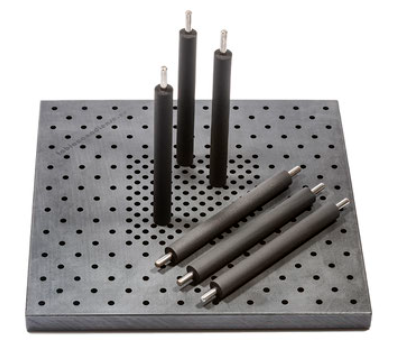
\includegraphics[width=0.5\linewidth]{img/Tabla_Canadiense.png}
        \caption{Tabla canadiense. Fuente tablacanadiense.es}
        \label{fig:tabla canadiense}
    \end{figure}

\section{Estado del arte.}

El proyecto ha de comenzar con búsqueda en el panorama actual en la medida de fuerza. 

En esta subsección se analiza y sintetiza el conocimiento existente en el área específica del proyecto. El objetivo principal es situar el trabajo dentro de un marco teórico y tecnológico, analizando investigaciones previas, aportes y detectando problemas que se puedan resolver.
\subsection{Dinamómetros:}
En la actualidad, los dinamómetros son una de las herramientas más utilizadas  para la medida de fuerza de los pacientes durante las sesiones de terapia ocupacional, fisioterapia o medicina deportiva. Existen diferentes modelos en el mercado que se diferencian en precisión, tecnología, precio o aplicación. 
A continuación, he destacado algunos de ellos:
\begin{itemize}
    \item Activforce 2: Es un dispositivo portátil e inalámbrico creado por la empresa estadounidense Activforce, con sede en California. Combina un dinamómetro con un inclinómetro lo que permite medir la fuerza máxima,promedio, rango de movimiento y simetría derecha-izquierda tanto en fuerza como en movimiento.Todas las mediciones se registran en una aplicación compatible con Android e iOS, donde el usuario puede ver toda la información recabada por el dispositivo.\cite{activforce}\footnote{Página web del dinamómetro Activforce2 con la información general del producto \cite{activforce}.}
    
    En la \textit{Figura} \ref{fig:activforce} se puede ver una imagen del producto.
    \begin{figure}[h]
        \centering
        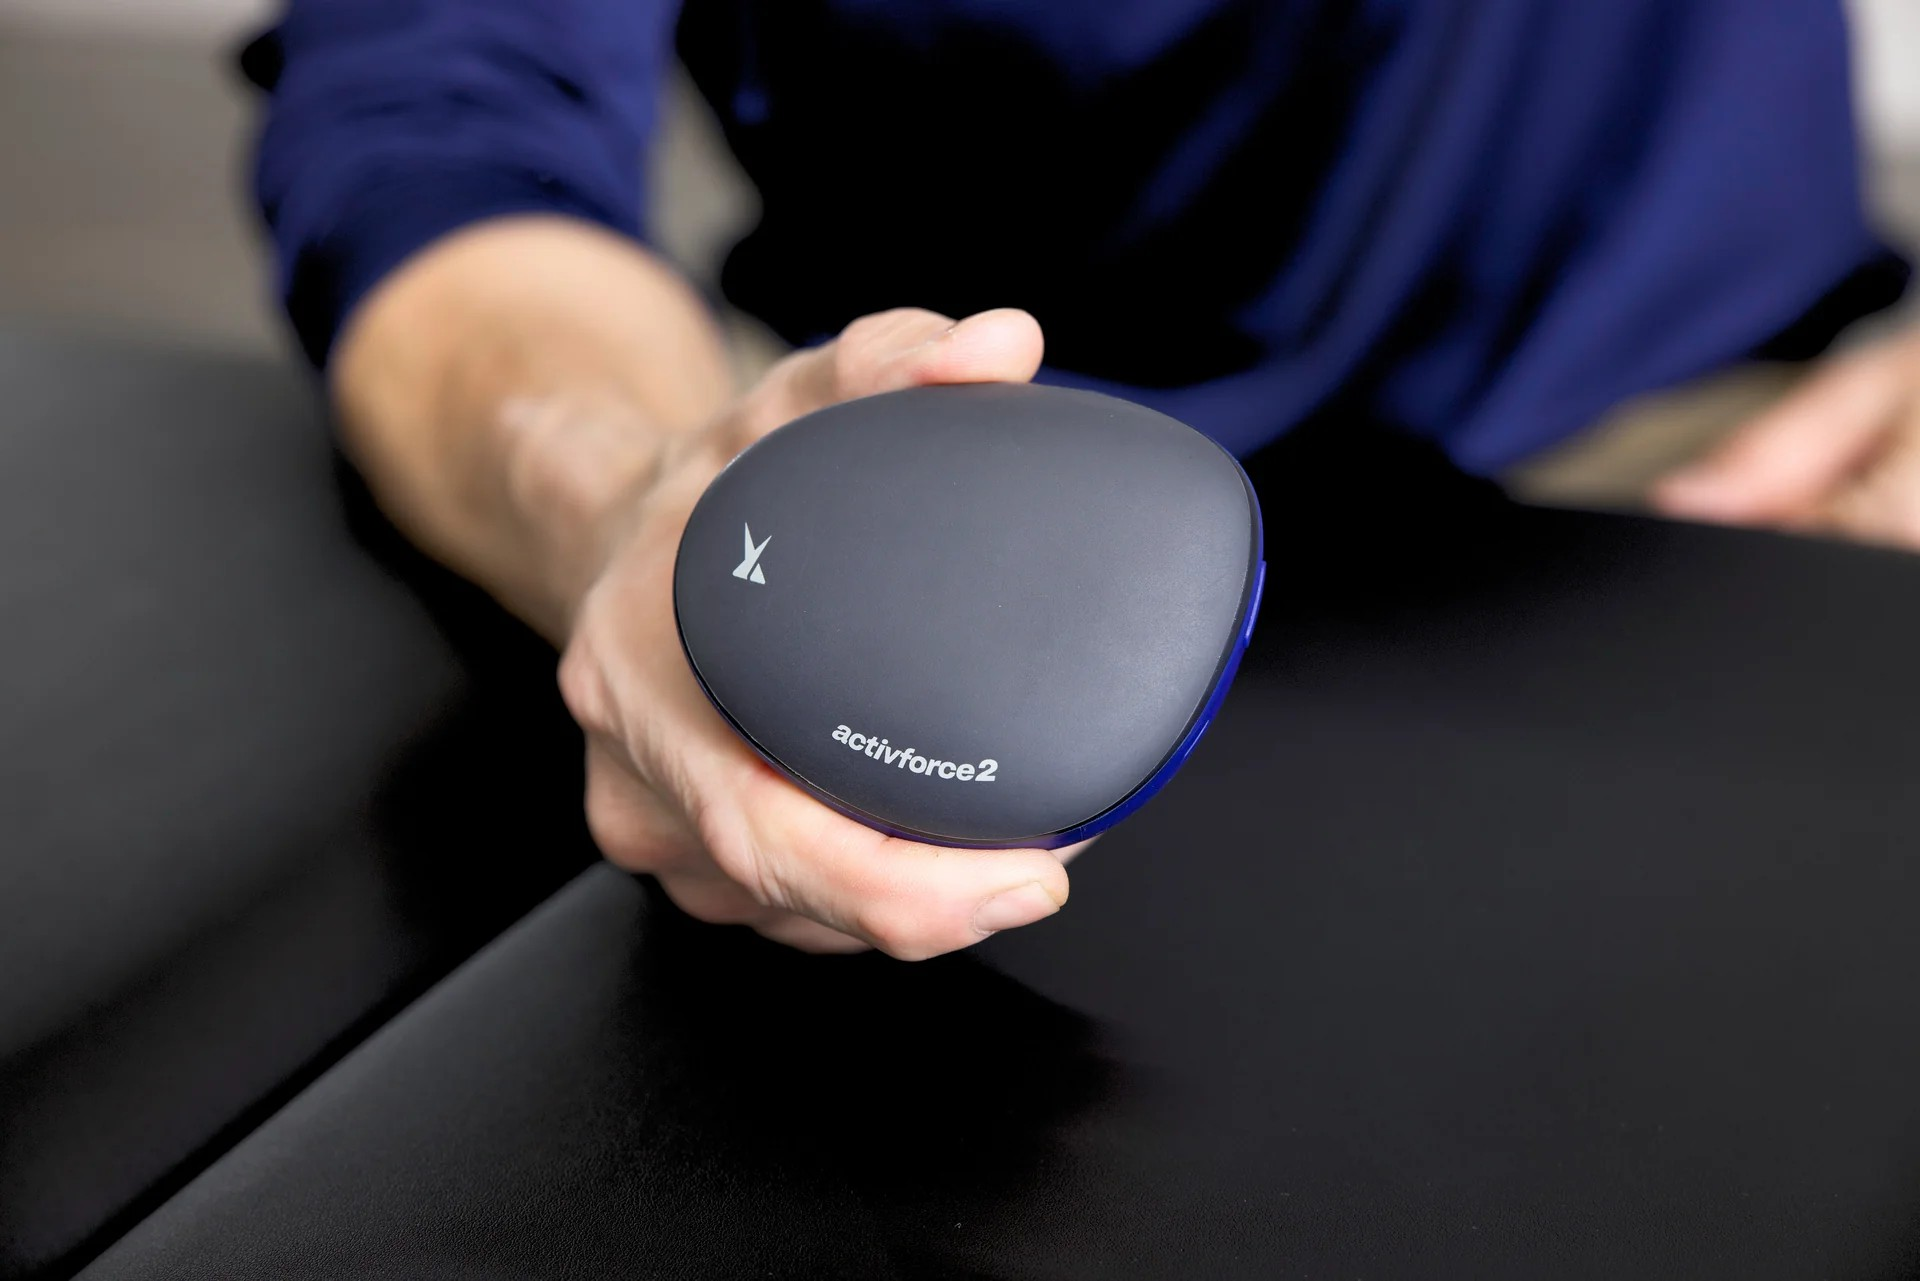
\includegraphics[width=0.5\textwidth]{img/ActivForce_Device.jpg}
        \caption{Dispositivo ActivForce2. Fuente activforce.com}
        \label{fig:activforce}
    \end{figure}
    
    Además, el Activforce 2 incluye varios accesorios que facilitan su uso en diferentes partes del cuerpo, permitiendo la ejecución de una amplia variedad de ejercicios y evaluaciones. Es un dispositivo de compra libre cuyo precio ronda los 450€. En la \textit{Figura} \ref{fig:activforce_Attachments} se puede ver una imagen del producto y los accesorios.
    \begin{figure}[h]
        \centering
        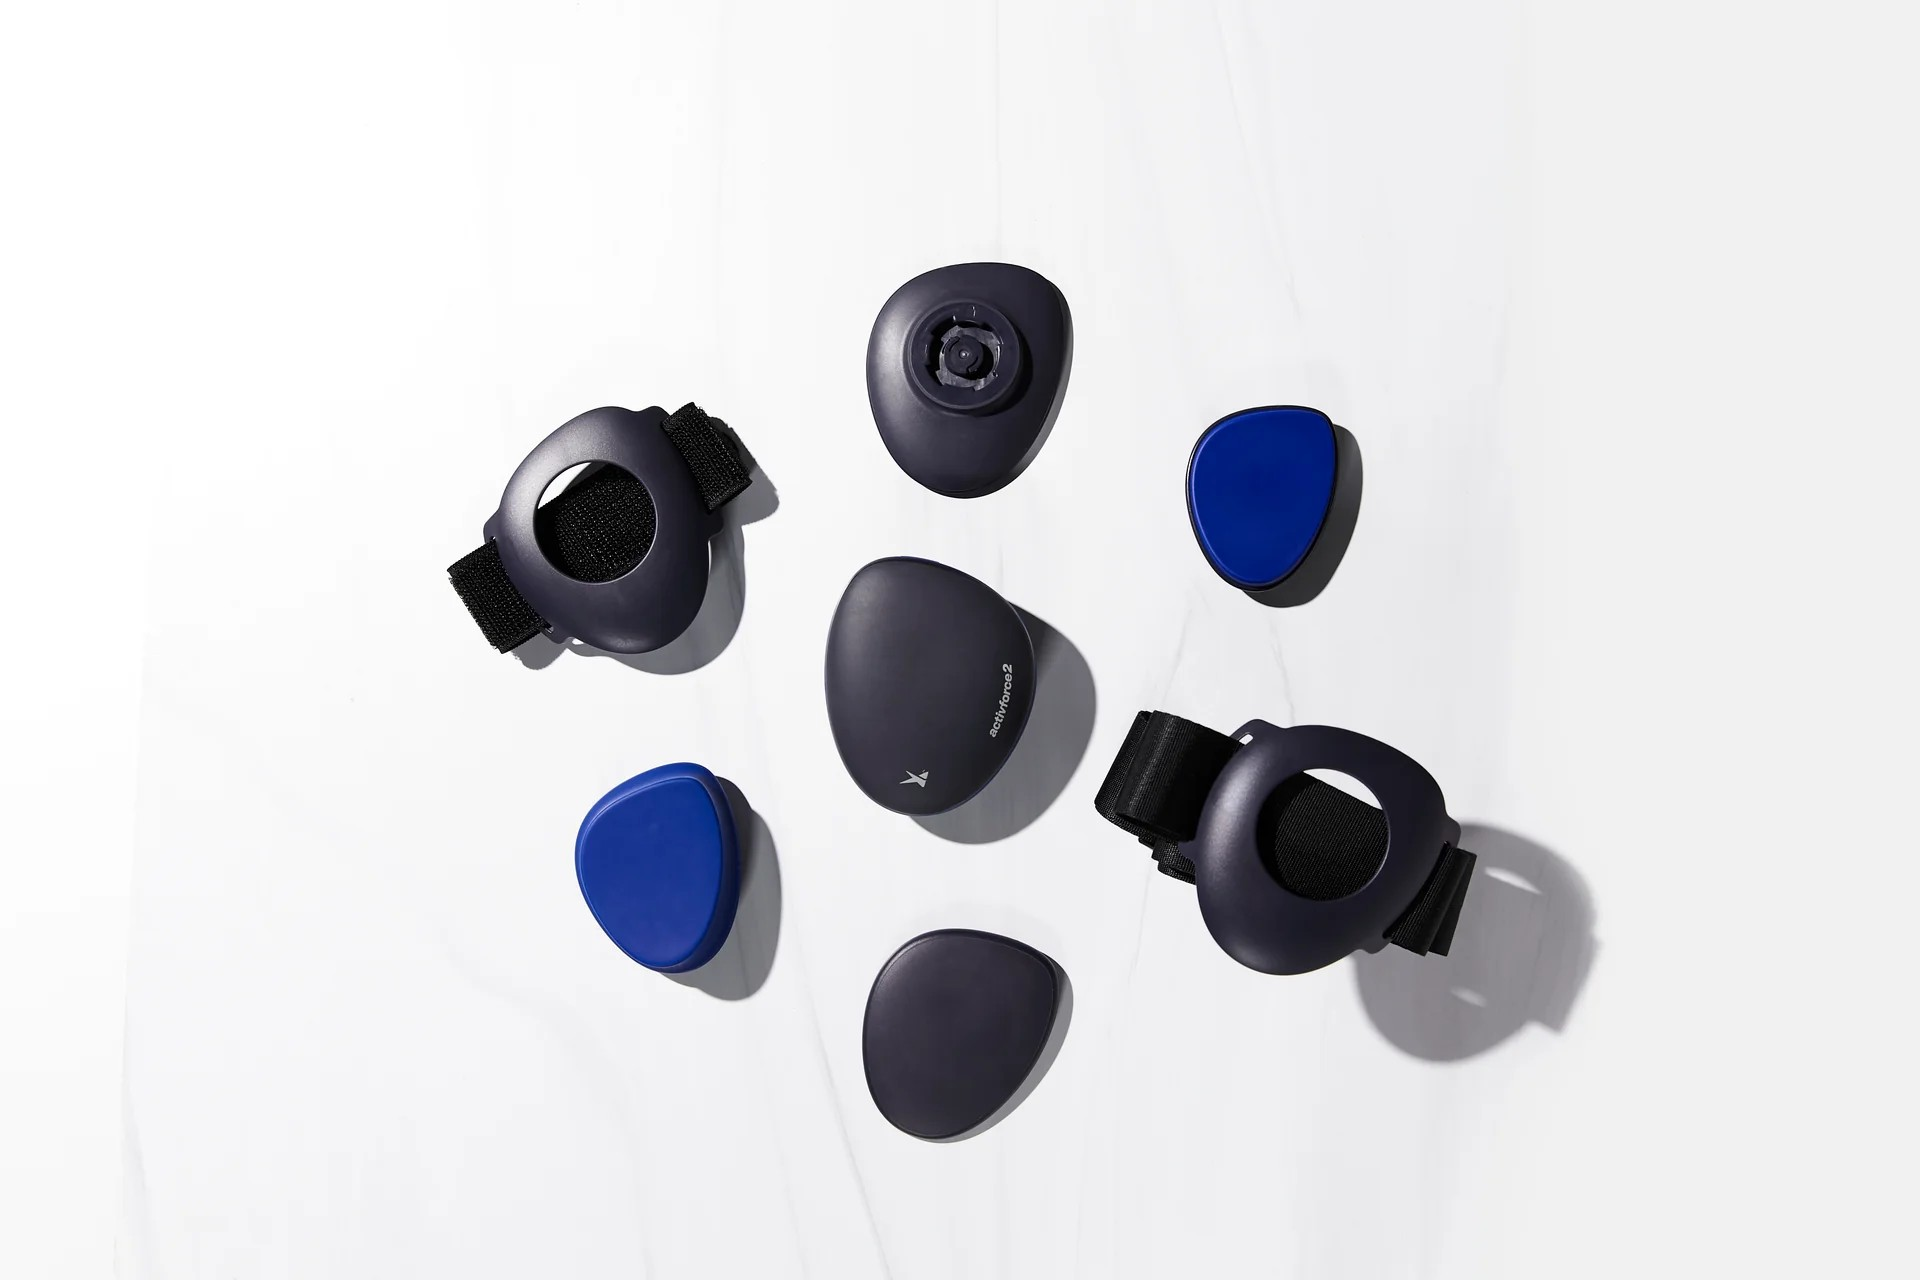
\includegraphics[width=0.5\textwidth]{img/ActivForce_Attachments.jpg}
        \caption{Accesorios compatibles con el dispositivo ActivForce2. Fuente activforce.com}
        \label{fig:activforce_Attachments}
    \end{figure}

    \item MicroFET 2: Es un dispositivo portátil e inalámbrico creado por la empresa belga MVS in motion. Es un dinamómetro diseñado para la evaluación y prueba de fuerza permite tomar mediciones de prueba muscular objetivas, cuantificables y confiables. 
    Es utilizado para la ayuda en el diagnóstico, pronóstico y el tratamiento de trastornos musculares. Presenta una pantalla digital donde se puede observar el valor de las mediciones en tiempo real. \cite{microfet}\footnote{Página web del dinamómetro MicroFET2 con la información general del producto \cite{microfet}.}
    Es un dispositivo de compra libre cuyo precio ronda los 1200€. 
    
    En la \textit{Figura} \ref{fig:MicroFET 2} se puede ver una imagen del dispositivo.
    \begin{figure}[h]
        \centering
        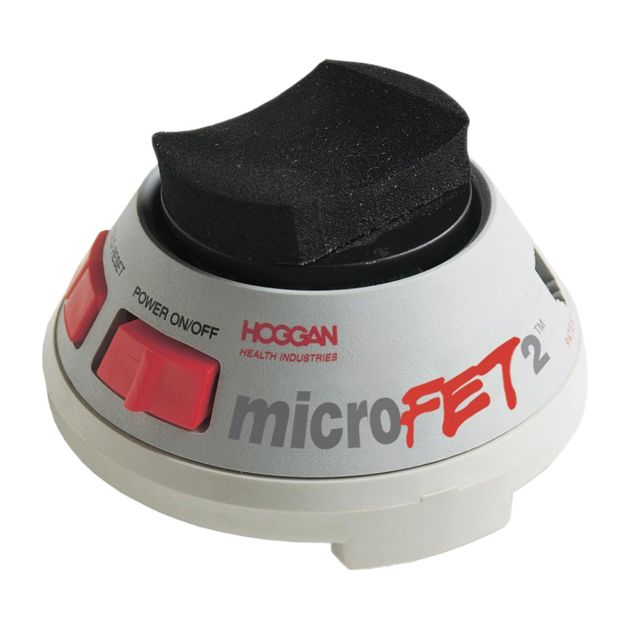
\includegraphics[width=0.45\textwidth]{img/MicroFET 2.jpg}
        \caption{Dispositivo MicroFET 2. Fuente fysiosupplies.es}
        \label{fig:MicroFET 2}
    \end{figure}
    
    \item MAP 80K1S: Es un dispositivo portátil e inalámbrico creado por la empresa alemana KERN \& SOHN. Es un dinamómetro de mano utilizado específicamente para tratamientos de rehabilitación, para la determinación de la fuerza de cierre de mano.
    Presenta cuatro modos de medición: tiempo real, valor máximo. valor promedio y de contaje. 
    Es utilizado en sesiones de rehabilitación para detectar la disminución de fuerza y la evolución del paciente entre sesiones. Cuenta con una pantalla digital donde se puede observar las mediciones realizadas. 
    Es un dispositivo de compra libre cuyo precio ronda los 280€. \cite{Map80k1s}\footnote{Página web del dinamómetro Map80K1S con la información general del producto \cite{Map80k1s}.}
    
    En la \textit{Figura} \ref{fig:Dispositivo MAP 80K1S} se puede ver una imagen del dispositivo.
      \begin{figure}[h]
        \centering
        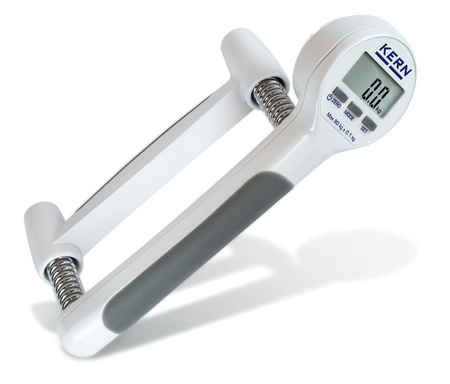
\includegraphics[width=0.5\textwidth]{img/MAP-80K1S.jpg}
        \caption{Dispositivo MAP 80K1S. Fuente kern-sohn.com}
        \label{fig:Dispositivo MAP 80K1S}
    \end{figure}
    
    \item Squeezy dynamometer: Es un dispositivo portátil, un dinamómetro de presión hidráulica de mano cuya medición se realiza apretando la perilla, generando presión que se transfiere al calibrador, el cual muestra con precisión la fuerza ejercida. Es un dispositivo de compra libre cuyo precio ronda los 70 €. \cite{SqueezeDinamometro}\footnote{Página web del dinamómetro Squeezy con la información general del producto \cite{SqueezeDinamometro}.} 
    
    En la \textit{Figura \ref{fig:Dinamómetro de Pera}} se puede ver una imagen del dispositivo.
    \begin{figure}[h]
        \centering
        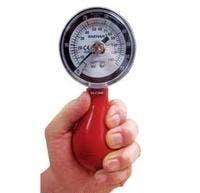
\includegraphics[width=0.5\textwidth]{img/Dinamometro pera.jpeg}
        \caption{Dinamómetro de Pera. Fuente rehabmedic.com}
        \label{fig:Dinamómetro de Pera}
    \end{figure}
\end{itemize}
\subsection{Artículos relacionados:}
La cuantificación de la fuerza en las manos  y su posterior análisis, es un tema que ya ha sido tratado por otros equipos de investigación en varios países. 

En esta subsección presentaré los artículos que he encontrado relacionados con el área, abarcando tanto la creación de dispositivos para la medición de la fuerza como el uso de dinamómetros para el registro de la evolución de los pacientes.
\begin{itemize}
    \item \textbf{Dispositivo de medición de fuerza de los dedos y su
rol en el seguimiento de las funciones de la mano}

Juliana Gomez et al, en su artículo llamado 'Dispositivo de medición de fuerza de los dedos y su rol en el seguimiento de las funciones de la mano' publicado en la revista de cirugía plástica Ibero Latinoamericana aborda la creación de un dispositivo capaz de medir la fuerza de los dedos de manera individual, para su uso en la evaluación del paciente sano y de pacientes con patologías traumáticas y no traumáticas, para determinar grados de discapacidad, seguimiento de enfermedades y/o recuperaciones. 
Este dispositivo se basa en el uso de 5 sensores del tipo Flexiforce A301 de la empresa TESKA®, sistema embebido
tipo Arduino y Matlab, se puede observar en la \textit{Figura \ref{fig:Dinamómetro creado por Juliana Gomez}}. Además, afirman la validez de su uso tras realizar un estudio con veinte sujetos sanos, obteniendo tasas de medición equiparables a las de otros sistemas.\cite{GOMEZ2022}\footnote{Artículo de la creación de un dispositivo con sensores de fuerza\cite{GOMEZ2022}.}
    \begin{figure}[h]
        \centering
        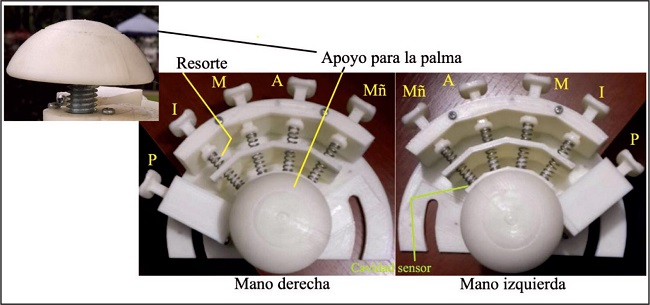
\includegraphics[width=0.7\textwidth]{img/dispositivo Revista.jpg}
        \caption{Dinamómetro creado por Juliana Gomez. Fuente scielo.isciii.es}
        \label{fig:Dinamómetro creado por Juliana Gomez}
    \end{figure}
\item \textbf{Uso del dinamómetro para mejorar la fuerza de la mano del adulto mayor.}
    
Mayra Lasteña Millingalli Ortega et al, en su artículo de revisión llamado 'Uso del dinamómetro para mejorar la fuerza de la mano del adulto mayor' publicado en la Revista Científica Arbitrada Multidisciplinaria PENTACIENCIAS en Octubre de 2023, realizan un trabajo de investigación revisando artículos en inglés y español publicados entre 2013 y 2022.
La población de estudio son pacientes geriátricos tratados en Terapia Ocupacional, las investigadoras exponen que actualmente en estas sesiones de terapia los pacientes son evaluados mediante métodos manuales como las escalas de registros, afirman que estos métodos son rudimentarios y no evidentes. \cite{Articulo_din}\footnote{Artículo que habla sobre el uso del dinamómetro\cite{Articulo_din}.}
\item \textbf{Diseño de dinamómetro con enfoque al monitoreo de fuerza de agarre de mano, en la 'Clínica Niño Sano' de niños quemados.}

    Tesis realizada en la universidad de Guatemala por Luis Carlos Ralon Gordillo en 2019, alumno del grado de  Ingeniería Mecatrónica. 

    Su tesis se fundamenta en la creación de un dispositivo para el monitoreo de la recuperación de la fuerza motriz de niños con quemaduras de tercer grado en la mano, utilizando un sensor de fuerza resistiva y un  microcontrolador PIC 16F88.

    En la \textit{Figura} \ref{fig:Prototipo dinamómetro Luis} se puede observar el prototipo realizado por el alumno.

    En el Luis Carlos Ralon afirma el correcto funcionamiento de su dispositivo, teniendo el sensor un  error promedio de 5.50 \%.

    \begin{figure}
        \centering
        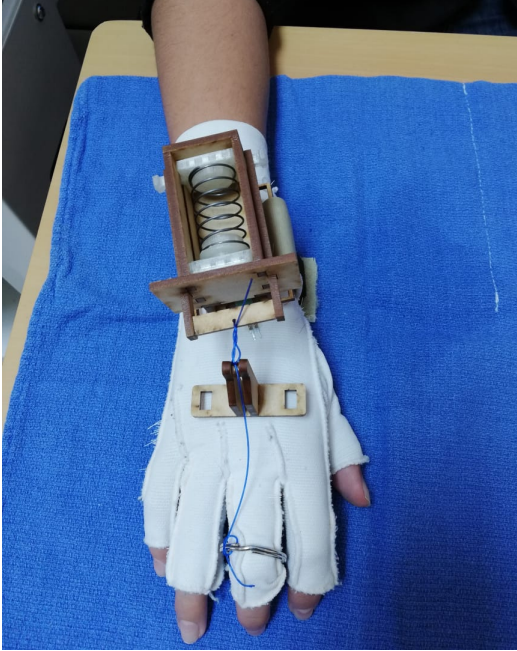
\includegraphics[width=0.5\linewidth]{img/TesisGuatemala.png}
        \caption{Prototipo dinamómetro Luis Carlos Ralon. Fuente Universidad del Valle de Guatemala }
        \label{fig:Prototipo dinamómetro Luis}
    \end{figure}    
\end{itemize}